\renewcommand{\lecturetitle}{Black-box NAS optimizers}
\renewcommand{\lecturetime}{Week 9, Video 3}
\section{\lecturetitle}
%-------------------------------------------------
%-------------------------------------------------
\myframe{Reinforcement Learning \litw{\href{https://arxiv.org/abs/1611.01578}{Zoph \& Le, 2017}}}{

{\begin{center}
	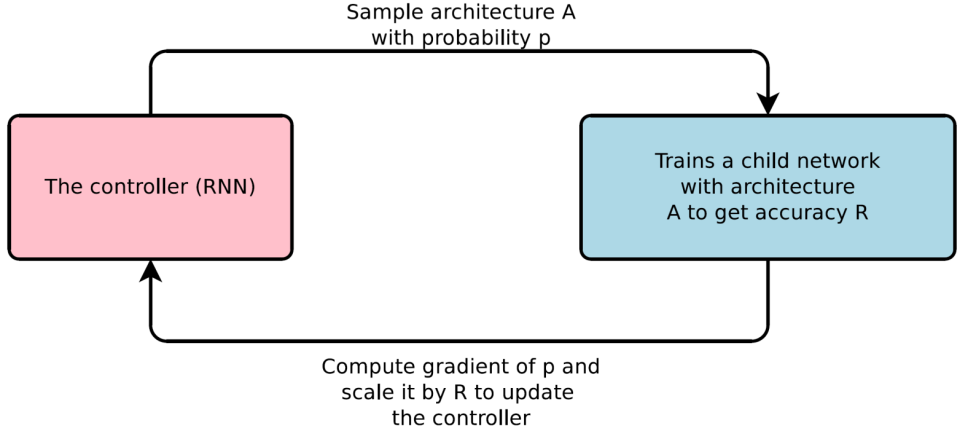
\includegraphics[width=.7\textwidth]{images/s27}
 \end{center}
}
\medskip
\begin{itemize}
	\item Use RNN ("\alert{Controller}") to generate a NN architecture piece-by-piece
	\item Train this NN ("\alert{Child Network}") and evaluate it on a validation set
	\item Use \alert{Reinforcement Learning (RL)} to update the parameters of the Controller 
	RNN to optimize the performance of the child models
\end{itemize}

}
%----------------------------------------------------------------------

%----------------------------------------------------------------------
\myframe{Learning CNNs with RL \litw{\href{https://arxiv.org/abs/1611.01578}{Zoph \& Le, 2017}}}{

\centering
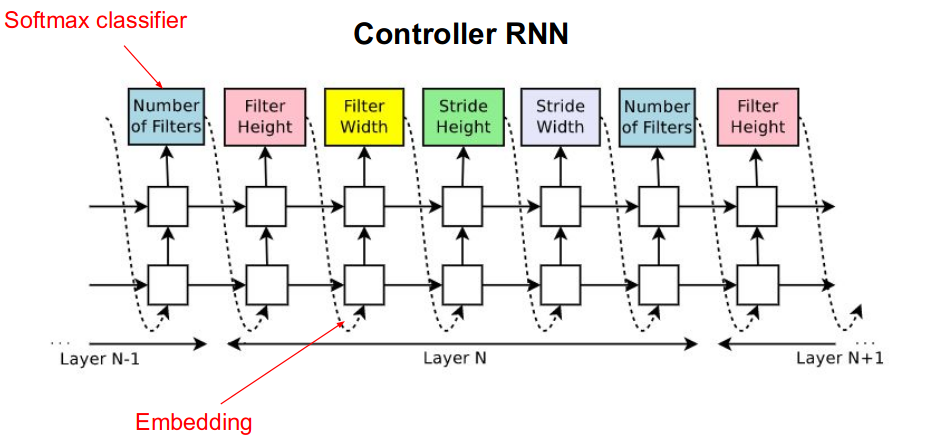
\includegraphics[width=.65\textwidth]{images/RL_CNN_controller}

\footnotesize{
	\myit{
	%	\item Maximize expected reward (validation accuracy): 
	%	$J(\theta_c)=E_{P(a_{1:T; \theta_c})}[R]$
		\item For a fixed number of layers, select:
		\begin{itemize}
			\item[-] \footnotesize Filter width/height, stride width/height, number of filters	
		\end{itemize}
	
	\pause
	\smallskip
		\item Large computational demands \alert{(800 GPUs for 2 weeks, 12.800 architectures evaluated)}
		%\myit{
		%	\item[-] \alert{800 GPUs for 2 weeks, 12.800 architectures evaluated}
		%}

	\pause
	\smallskip
	%	\item Each child model was trained for 50 epochs
	%	\item The final chosen architecture is trained for longer (600 epochs)
		%, optimizing the weights with SGD
		\item \alert{State-of-the-art results for CIFAR-10 \& Penn Treebank architecture}
		\myit{
			\item[$\rightarrow$] \footnotesize Brought NAS into the limelight
		}
	}
	}
}
%----------------------------------------------------------------------

%----------------------------------------------------------------------

\myframetop{Learning CNN cells with RL \litw{\href{http://openaccess.thecvf.com/content_cvpr_2018/html/Zoph_Learning_Transferable_Architectures_CVPR_2018_paper.html}{Zoph et al. ’18}}}{
	\centering
	
	\begin{itemize}
		\item 2 types of cells: normal and reduction cells
		\item For each type of cell: $B$ blocks, each with 5 choices
		\myit{
			\item[-] Choose two previous feature maps (from this cell)
			\item[-] For each of these, choose an operation (3$\times$3 conv, max-pool, etc.)
			\item[-] Choose a merge operation to combine the two results (concat or add)
		}
	
	\end{itemize}
	\bigskip
	\bigskip
	\smallskip
	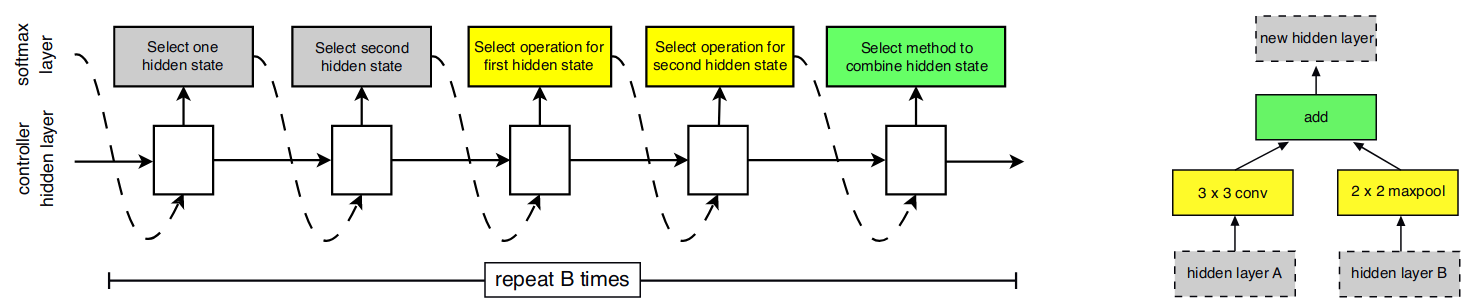
\includegraphics[width=\textwidth]{images/RL_conv_cell}
	%\pause
	%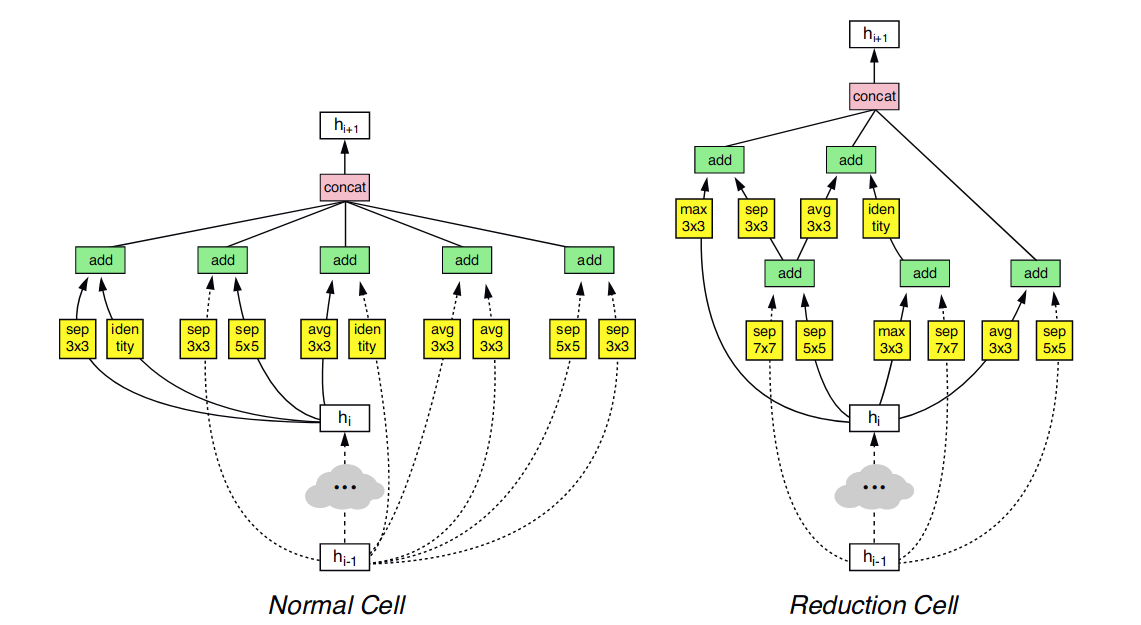
\includegraphics[width=.5\textwidth]{images/RL_normal_reduction}
	
}
%----------------------------------------------------------------------
%----------------------------------------------------------------------

\myframetop{NAS as Hyperparameter Optimization}{
	\begin{itemize}
		\item 2 types of cells: normal and reduction cells
		\item For each type of cell: $B$ blocks, each with 5 choices
		\myit{
			\item[-] Choose two previous feature maps (from this cell)
			\item[-] For each of these, choose an operation (3$\times$3 conv, max-pool, etc.)
			\item[-] Choose a merge operation to combine the two results (concat or add)
		}
	
	\end{itemize}
	\bigskip
	
	\begin{itemize}
	  \item This can be modelled as a HPO problem with 2$\times$5$\times$B variables:
	\end{itemize}
	~~~~~~\hspace*{0.08cm}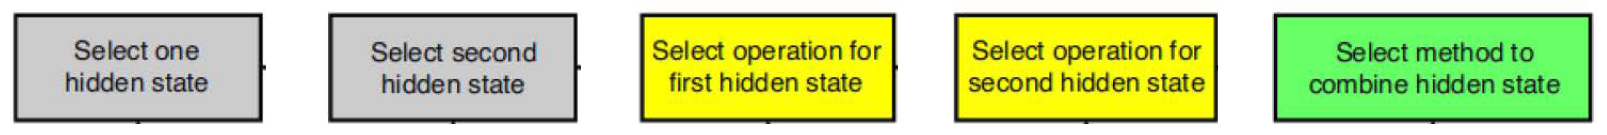
\includegraphics[width=0.613\textwidth]{images/NAS-RL-space_as_HPO}
	
}

%----------------------------------------------------------------------
%----------------------------------------------------------------------

\myframe{Evolution}{

\centering
\begin{enumerate}
	\footnotesize
	\item Initialize a \alert{population} of randomly sampled architectures.
	\item Sample pairs and select the architecture to mutate based on the \emph{fitness} function (e.g. validation error). \alert{Remove} the other from the population.
	\item Apply \alert{mutation} steps to the selected architecture, such as adding, changing or removing a layer. Add the new child architecture to the population. \lit{\href{https://arxiv.org/abs/1703.01041}{Real et al. 2017}; \href{https://openreview.net/forum?id=BJQRKzbA-}{Liu et al. 2017}; \href{https://arxiv.org/pdf/1703.00548.pdf}{Miikkulainen et al. 2017}}
\end{enumerate}

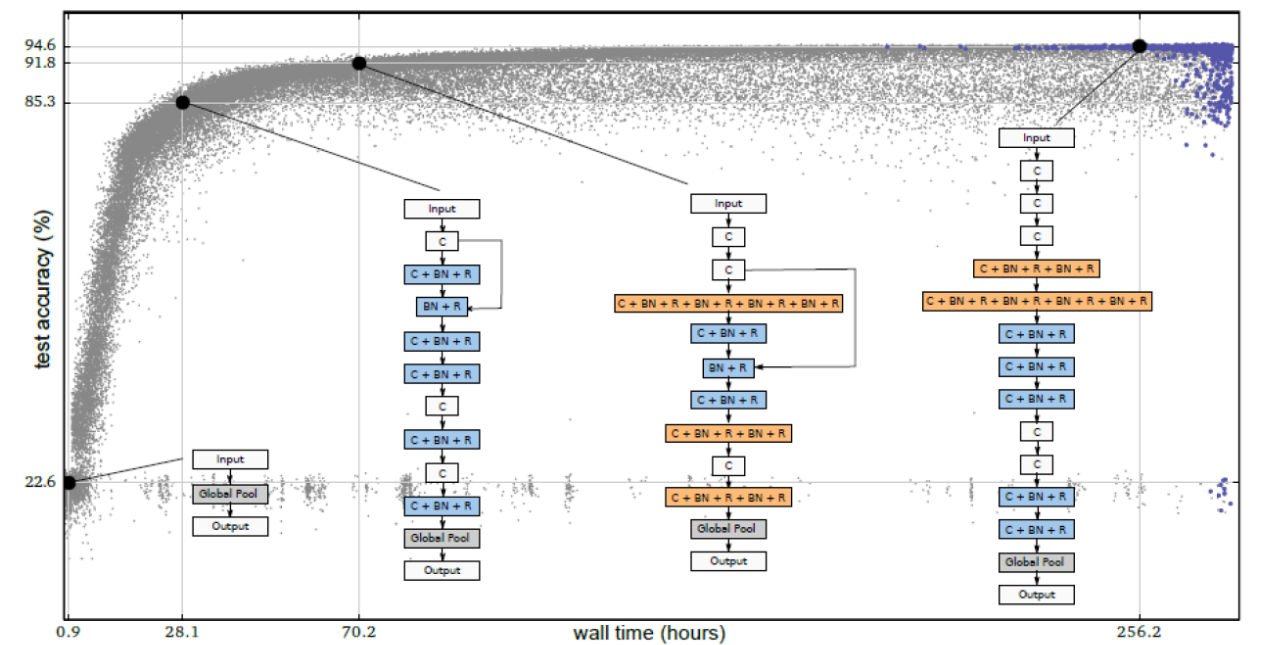
\includegraphics[width=.7\textwidth]{images/neuroevolution.png}\\

}
%----------------------------------------------------------------------

%----------------------------------------------------------------------
\myframe{Regularized/Aging Evolution \litw{\href{https://arxiv.org/abs/1802.01548}{Real et al, 2019}}}{

\centering
\begin{itemize}
	\footnotesize
	\item Standard evolutionary algorithm, but oldest solutions are dropped from
	population, instead of the worst.
	\item \alert{Evolution only for architectures; standard SGD for training weights}
	\item \alert{Same fixed-length (HPO) search space} as used for RL \lit{\href{http://openaccess.thecvf.com/content_cvpr_2018/html/Zoph_Learning_Transferable_Architectures_CVPR_2018_paper.html}{Zoph et al. ’18}}
\end{itemize}

\bigskip
\begin{columns}[T]

\column{0.4\textwidth}
\onslide<2->{
\centering
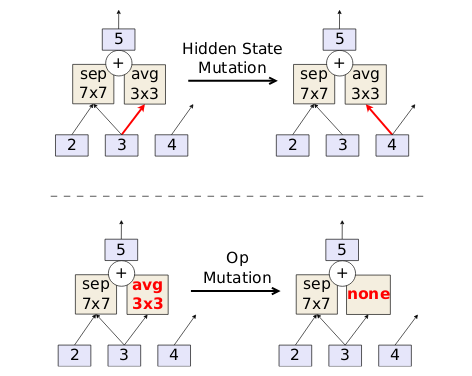
\includegraphics[width=\textwidth]{images/aging_evolution_mutations.png}
\footnotesize{Different types of mutations in cell search space}
}
\column{0.4\textwidth}
\onslide<3->{
\centering
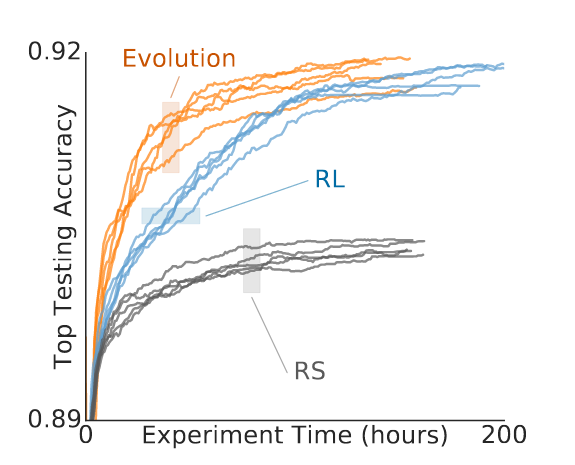
\includegraphics[width=.9\textwidth]{images/aging_evolution_results.png}
\footnotesize{State-of-the-art performance in apples-to-apples comparison\\ $\rightarrow$ \alert{AmoebaNet}}
}
\end{columns}

}
%----------------------------------------------------------------------

%----------------------------------------------------------------------
\myframe{Bayesian Optimization (BO)}{
	\myit{
		\item Encode the architecture as a vector space (like regularized evolution)
		\lit{\href{http://proceedings.mlr.press/v28/bergstra13.pdf}{Bergstra et al. 2013}, \href{https://ml.informatik.uni-freiburg.de/papers/15-IJCAI-Extrapolation_of_Learning_Curves.pdf}{Domhan et al. 2015}, \href{https://ml.informatik.uni-freiburg.de/papers/16-AUTOML-AutoNet.pdf}{Mendoza et al. 2015}, \href{https://arxiv.org/abs/1807.06906}{Zela et al. 2018}}
\pause
\medskip
		\item Joint optimization of architecture and hyperparameters, already in Auto-Net \lit{\href{https://ml.informatik.uni-freiburg.de/papers/16-AUTOML-AutoNet.pdf}{Mendoza et al. 2016}}
		\myit{
			\item[-] Based on BO with a random forest model (SMAC \lit{\href{https://ml.informatik.uni-freiburg.de/papers/11-LION5-SMAC.pdf}{Hutter et al, 2011}}) 
			\item[-] \alert{First automated deep learning (Auto-DL) method to win a machine learning competition dataset against human experts}
		}
\pause
\medskip
		\item Kernels for GP-based NAS
		\myit{
			\item[-] Arc kernel \lit{\href{https://ml.informatik.uni-freiburg.de/papers/13-BayesOpt_Arc-Kernel.pdf}{Swersky et al, 2013}}
			\item[-] NASBOT \lit{\href{https://arxiv.org/abs/1802.07191}{Kandasamy et al, 2018}}
		}
\pause
\medskip		
		\item There are also several recent promising BO approaches based on neural networks
	}
}
%-----------------------------------------------------------------------

%----------------------------------------------------------------------
\myframe{Case study: NASBOT \litw{\href{https://arxiv.org/abs/1802.07191}{Kandasamy et al., NeurIPS 2018}}}{

\centering
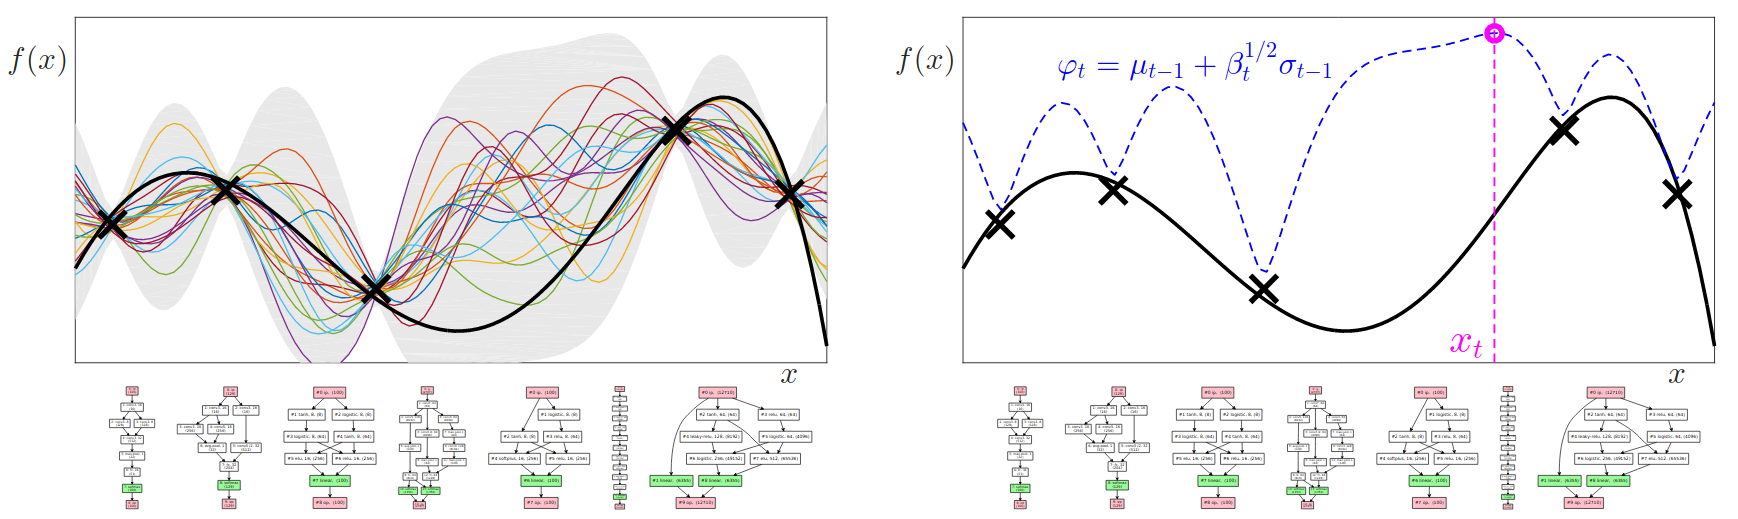
\includegraphics[width=.9\textwidth]{images/nasbot_1.png}
\myit{
\footnotesize
		\item Gaussian Process BO is not that straighforward in non-Euclidian spaces such as the space of neural architectures
		\myit{
		\footnotesize
			\item How to define a kernel (which entails the distance) in the architecture space?
			\item How to optimize the acquisition function?
		}
\pause
\medskip
		\item \alert{NASBOT}
		\myit{
		\footnotesize
			\item defines a distance metric based on Optimal Transport (\alert{OTMANN})
			\item optimizes the acquisition function using \alert{evolution}
			
		}		
}

}

%----------------------------------------------------------------------
\myframe{Case study: NASBOT \litw{\href{https://arxiv.org/abs/1802.07191}{Kandasamy et al., NeurIPS 2018}}}{

\centering

\begin{columns}
\column{.6\textwidth}
\vspace{-7cm}
\myit{
		\item The kernel: $\kappa = e^{-\beta d^{p}}$, where $d$ is the OTMANN distance
		\myit{
			\item[--] To compute $d$ between two architectures $G_1$, $G_2$: match computation (layer mass) in layers in $G_1$ to $G_2$
		}
}
\pause
\medskip

\myit{
	\item $Z \in \mathtt{R}^{n_1 \times n_2}$
	\myit{
		\item $Z_{ij} \longleftarrow$ \alert{amount of matched mass} between layer $i\in G_1$ and $j \in G_2$
	}
	\medskip
	\item $d \triangleq \argminA_Z \phi_{lmm}(Z) + \phi_{str}(Z) + \phi_{nas}(Z)$
	\myit{
		\item[--] $\phi_{lmm}(Z)$: label mismatch penalty
		\item[--] $\phi_{str}(Z)$: structural penalty
		\item[--] $\phi_{nas}(Z)$: non-assignment penalty
	}

}

\column{.4\textwidth}
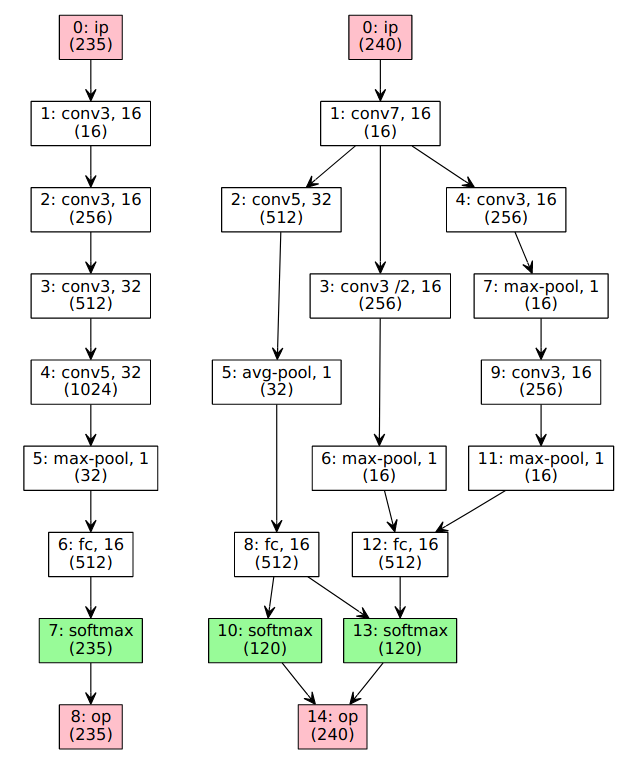
\includegraphics[width=\textwidth]{images/nasbot_2.png}

\end{columns}

}
%-----------------------------------------------------------------------

%----------------------------------------------------------------------
\myframe{Questions to Answer for Yourself / Discuss with Friends}{

	\myit{
		\item Repetition:\\ 
		\alert{What are some pros and cons of using black-box optimizers for NAS?}
		\item Repetition:\\
		\alert{How can NAS be modelled as an HPO problem in the Euclidian space?}
\medskip
		\item Discussion:\\ \alert{Why does discarding the oldest individual rather than the worse help in Regularized/Aging evolution?}
	}	 
}
%-----------------------------------------------------------------------

